%%
%% This is file `sample-manuscript.tex',
%% generated with the docstrip utility.
%%
%% The original source files were:
%%
%% samples.dtx  (with options: `all,proceedings,bibtex,manuscript')
%%
%% IMPORTANT NOTICE:
%%
%% For the copyright see the source file.
%%
%% Any modified versions of this file must be renamed
%% with new filenames distinct from sample-manuscript.tex.
%%
%% For distribution of the original source see the terms
%% for copying and modification in the file samples.dtx.
%%
%% This generated file may be distributed as long as the
%% original source files, as listed above, are part of the
%% same distribution. (The sources need not necessarily be
%% in the same archive or directory.)
%%
%%
%% Commands for TeXCount
%TC:macro \cite [option:text,text]
%TC:macro \citep [option:text,text]
%TC:macro \citet [option:text,text]
%TC:envir table 0 1
%TC:envir table* 0 1
%TC:envir tabular [ignore] word
%TC:envir displaymath 0 word
%TC:envir math 0 word
%TC:envir comment 0 0
%%
%%
%% The first command in your LaTeX source must be the \documentclass
%% command.
%%
%% For submission and review of your manuscript please change the
%% command to \documentclass[manuscript, screen, review]{acmart}.
%%
%% When submitting camera ready or to TAPS, please change the command
%% to \documentclass[sigconf]{acmart} or whichever template is required
%% for your publication.
%%
%%
\documentclass[manuscript,screen,review,anonymous]{acmart}
% \documentclass[acmsmall,sigconf]{acmart}

%%
%% \BibTeX command to typeset BibTeX logo in the docs
\AtBeginDocument{%
  \providecommand\BibTeX{{%
    Bib\TeX}}}

% %% Rights management information.  This information is sent to you
% %% when you complete the rights form.  These commands have SAMPLE
% %% values in them; it is your responsibility as an author to replace
% %% the commands and values with those provided to you when you
% %% complete the rights form.
% \setcopyright{acmlicensed}
% \copyrightyear{2018}
% \acmYear{2018}
% \acmDOI{XXXXXXX.XXXXXXX}

% %% These commands are for a PROCEEDINGS abstract or paper.
% \acmConference[Conference acronym 'XX]{Make sure to enter the correct
%   conference title from your rights confirmation emai}{June 0--05,
%   2018}{Woodstock, NY}
% %%
% %%  Uncomment \acmBooktitle if the title of the proceedings is different
% %%  from ``Proceedings of ...''!
% %%
% %%\acmBooktitle{Woodstock '18: ACM Symposium on Neural Gaze Detection,
% %%  June 03--05, 2018, Woodstock, NY}
% \acmISBN{978-1-4503-XXXX-X/18/06}


%%
%% Submission ID.
%% Use this when submitting an article to a sponsored event. You'll
%% receive a unique submission ID from the organizers
%% of the event, and this ID should be used as the parameter to this command.
%%\acmSubmissionID{123-A56-BU3}

%%
%% For managing citations, it is recommended to use bibliography
%% files in BibTeX format.
%%
%% You can then either use BibTeX with the ACM-Reference-Format style,
%% or BibLaTeX with the acmnumeric or acmauthoryear sytles, that include
%% support for advanced citation of software artefact from the
%% biblatex-software package, also separately available on CTAN.
%%
%% Look at the sample-*-biblatex.tex files for templates showcasing
%% the biblatex styles.
%%

%%
%% The majority of ACM publications use numbered citations and
%% references.  The command \citestyle{authoryear} switches to the
%% "author year" style.
%%
%% If you are preparing content for an event
%% sponsored by ACM SIGGRAPH, you must use the "author year" style of
%% citations and references.
%% Uncommenting
%% the next command will enable that style.
%%\citestyle{acmauthoryear}

\usepackage{mathtools}
\usepackage{multirow}
\usepackage{subcaption}

\graphicspath{{images/}}
\DeclareGraphicsExtensions{.pdf}

\DeclarePairedDelimiter{\set}{\{}{\}}
\DeclarePairedDelimiter{\tuple}{(}{)}
\DeclarePairedDelimiter{\abs}{\lvert}{\rvert}
\renewcommand{\implies}{\rightarrow}
\newcommand{\db}{D}
\newcommand{\dbs}{\mathcal{D}}
\newcommand{\model}{\mathcal{M}}
\newcommand{\priv}{R}
\newcommand{\pos}{\hat{P}}
\newcommand{\posm}{\hat{P}_\mathcal{M}}
\newcommand{\tru}{T}
\newcommand{\leg}{L}
\newcommand{\sco}{\hat{S}}
\newcommand{\scom}{\hat{S}_\mathcal{M}}
\newcommand{\calib}{C}
\newcommand{\prob}[1]{\text{Pr}[#1]}
\newcommand{\mi}[2]{I(#1;#2)}
\newcommand{\entropy}[1]{H(#1)}

%%
%% end of the preamble, start of the body of the document source.
\begin{document}

%%
%% The "title" command has an optional parameter,
%% allowing the author to define a "short title" to be used in page headers.
\title{Quantitative Auditing of Fairness Measures with Differentially Private Synthetic Data}

%%
%% The "author" command and its associated commands are used to define
%% the authors and their affiliations.
%% Of note is the shared affiliation of the first two authors, and the
%% "authornote" and "authornotemark" commands
%% used to denote shared contribution to the research.
\author{Chih-Cheng Rex Yuan}
\email{hello@rexyuan.com}
\affiliation{%
  \institution{Institute of Information Science, Academia Sinica}
  \city{Taipei}
  \country{Taiwan}
}

\author{Bow-Yaw Wang}
\email{bywang@iis.sinica.edu.tw}
\affiliation{%
  \institution{Institute of Information Science, Academia Sinica}
  \city{Taipei}
  \country{Taiwan}
}

%%
%% By default, the full list of authors will be used in the page
%% headers. Often, this list is too long, and will overlap
%% other information printed in the page headers. This command allows
%% the author to define a more concise list
%% of authors' names for this purpose.
% \renewcommand{\shortauthors}{Trovato et al.}

%%
%% The abstract is a short summary of the work to be presented in the
%% article.
\begin{abstract}
  abstract
\end{abstract}

% %%
% %% The code below is generated by the tool at http://dl.acm.org/ccs.cfm.
% %% Please copy and paste the code instead of the example below.
\begin{CCSXML}
  <ccs2012>
     <concept>
         <concept_id>10002944.10011123.10011124</concept_id>
         <concept_desc>General and reference~Metrics</concept_desc>
         <concept_significance>500</concept_significance>
         </concept>
     <concept>
         <concept_id>10002978.10003029.10011703</concept_id>
         <concept_desc>Security and privacy~Usability in security and privacy</concept_desc>
         <concept_significance>500</concept_significance>
         </concept>
     <concept>
         <concept_id>10002951.10003227.10003351</concept_id>
         <concept_desc>Information systems~Data mining</concept_desc>
         <concept_significance>300</concept_significance>
         </concept>
     <concept>
         <concept_id>10010147.10010257</concept_id>
         <concept_desc>Computing methodologies~Machine learning</concept_desc>
         <concept_significance>300</concept_significance>
         </concept>
     <concept>
         <concept_id>10010147.10010178</concept_id>
         <concept_desc>Computing methodologies~Artificial intelligence</concept_desc>
         <concept_significance>300</concept_significance>
         </concept>
     <concept>
         <concept_id>10002978.10002991.10002995</concept_id>
         <concept_desc>Security and privacy~Privacy-preserving protocols</concept_desc>
         <concept_significance>300</concept_significance>
         </concept>
     <concept>
         <concept_id>10002951.10003227</concept_id>
         <concept_desc>Information systems~Information systems applications</concept_desc>
         <concept_significance>300</concept_significance>
         </concept>
     <concept>
         <concept_id>10002950.10003648.10003688.10003690</concept_id>
         <concept_desc>Mathematics of computing~Contingency table analysis</concept_desc>
         <concept_significance>300</concept_significance>
         </concept>
   </ccs2012>
\end{CCSXML}

\ccsdesc[500]{General and reference~Metrics}
\ccsdesc[500]{Security and privacy~Usability in security and privacy}
\ccsdesc[300]{Information systems~Data mining}
\ccsdesc[300]{Computing methodologies~Machine learning}
\ccsdesc[300]{Computing methodologies~Artificial intelligence}
\ccsdesc[300]{Security and privacy~Privacy-preserving protocols}
\ccsdesc[300]{Information systems~Information systems applications}
\ccsdesc[300]{Mathematics of computing~Contingency table analysis}
% %%
% \begin{CCSXML}
% <ccs2012>
%  <concept>
%   <concept_id>00000000.0000000.0000000</concept_id>
%   <concept_desc>Do Not Use This Code, Generate the Correct Terms for Your Paper</concept_desc>
%   <concept_significance>500</concept_significance>
%  </concept>
%  <concept>
%   <concept_id>00000000.00000000.00000000</concept_id>
%   <concept_desc>Do Not Use This Code, Generate the Correct Terms for Your Paper</concept_desc>
%   <concept_significance>300</concept_significance>
%  </concept>
%  <concept>
%   <concept_id>00000000.00000000.00000000</concept_id>
%   <concept_desc>Do Not Use This Code, Generate the Correct Terms for Your Paper</concept_desc>
%   <concept_significance>100</concept_significance>
%  </concept>
%  <concept>
%   <concept_id>00000000.00000000.00000000</concept_id>
%   <concept_desc>Do Not Use This Code, Generate the Correct Terms for Your Paper</concept_desc>
%   <concept_significance>100</concept_significance>
%  </concept>
% </ccs2012>
% \end{CCSXML}

% \ccsdesc[500]{Do Not Use This Code~Generate the Correct Terms for Your Paper}
% \ccsdesc[300]{Do Not Use This Code~Generate the Correct Terms for Your Paper}
% \ccsdesc{Do Not Use This Code~Generate the Correct Terms for Your Paper}
% \ccsdesc[100]{Do Not Use This Code~Generate the Correct Terms for Your Paper}

% %%
% %% Keywords. The author(s) should pick words that accurately describe
% %% the work being presented. Separate the keywords with commas.
% \keywords{Do, Not, Us, This, Code, Put, the, Correct, Terms, for,
%   Your, Paper}

% \received{20 February 2007}
% \received[revised]{12 March 2009}
% \received[accepted]{5 June 2009}

%%
%% This command processes the author and affiliation and title
%% information and builds the first part of the formatted document.
\maketitle

\section{Introduction}

\section{Related Work}

TODO: add more connections to our work

Fairness in machine learning has become a crucial area of research\cite{barocas2023fairness}. Various fairness measures have been proposed to quantify\cite{yeh2024analyzing} the fairness of AI models\cite{pessach2022review,corbett2017algorithmic,vzliobaite2017measuring,hardt2016equality,corbett2017algorithmic,berk2021fairness,chouldechova2017fair,kleinberg2016inherent}.

Auditing of AI models is an important step in ensuring that these models are fair\cite{ferrara2023fairness}. Different tools have been developed to check the fairness of AI models\cite{yuan2024ensuring,saleiro2018aequitas,bellamy2019ai,bird2020fairlearn}.

% differential privacy

Differential Privacy has risen to become the standard of privacy protection in many data analyses\cite{jiang2021applications}. It offers a formal framework for quantifying privacy guarantees when releasing information derived from sensitive data\cite{dwork2006calibrating,dwork2014algorithmic}.

Different flavors of Differential Privacy have been proposed over the years\cite{desfontaines2019sok}, such as Gaussian Differential Privacy\cite{dong2022gaussian}, Pufferfish Differential Privacy\cite{kifer2012rigorous}, Bayesian Differential Privacy\cite{triastcyn2020bayesian}, and R\'enyi Differential Privacy\cite{mironov2017renyi}.

% synthetic data

The generation of synthetic data\cite{raghunathan2021synthetic,lu2023machine} under Differential Privacy constraints allows for data sharing without compromising privacy\cite{tao2021benchmarking}. There have been several techniques developed for Differentially Private synthetic data generation\cite{rosenblatt2020differentially,fan2020relational,bowen2019comparative,bowen2020comparative,arnold2020really,xu2019modeling} in recent years.

TODO: some works aim to change properties of og data. we want to preserve. so we dont consider this case

There are also works that aim to introduce bias to synthetic data\cite{jiang2024synthetic,baumann2023bias}.

While helpful, there are some technical limitations\cite{stadler2022synthetic,cheng2021can,ganev2022robin,wyllie2024fairness} and ethical concerns\cite{whitney2024real} with the use of synthetic data.

\section{Preliminaries}
\label{sec:prelim}

Let $\prod_i x_i$ denote the Cartesian product of $x_i$s.

An \emph{attribute} is a symbol $A$.
The set of all attributes is $\mathcal{A}$.
An \emph{attribute value} is a symbol $a$.
The set of all attribute values is $\Omega$.
An \emph{attribute value space} is a function $\sigma : \mathcal{A} \implies 2^{\Omega}$
specifying the set of valid values that attributes can take on.
A \emph{row} with respect to $\sigma$
is a function $r : \mathcal{A} \implies \Omega$
where $r(A) \in \sigma(A)$.
The set of all rows is $\mathcal{R}$.
A \emph{database} is a tuple $\db =
\tuple{
    \mathcal{A}_{\db},
    \Omega_{\db},
    \sigma_{\db},
    \mathcal{R}_{\db}
}$
where
$\mathcal{A}_{\db} \subseteq \mathcal{A}$
is the set of attributes in $\db$,
$\Omega_{\db} \subseteq \Omega$
is the set of attribute values in $\db$,
$\sigma_{\db} : \mathcal{A}_{\db} \implies 2^{\Omega_{\db}}$
is the function specifying the valid values that each attribute can take on in $\db$,
and $\mathcal{R}_{\db} \subseteq \mathcal{R}$
is the set of rows with respect to $\sigma_{\db}$ in $\db$
with $r_\db : \mathcal{A}_\db \implies \Omega_\db$
for all $r_\db \in \mathcal{R}_\db$
and $r_\db(A) \in \sigma_\db(A)$
for all $A \in \mathcal{A}_\db$.
The set of all databases is $\dbs$.

Let $X \in \mathcal{X}$ be a discrete random variable and $p(x) := \prob{X = x}$. Its \emph{marginal Shannon entropy} is $\entropy{X} := -\sum_{x \in \mathcal{X}} p(x) \text{log} p(x)$. It quantifies the level of uncertainty of $X$. Let $Y \in \mathcal{Y}$ be another discrete random variable. Their \emph{joint Shannon entropy} is $\entropy{X,Y} := -\sum_{x \in \mathcal{X}} \sum_{y \in \mathcal{Y}} p(x, y) \text{log} p(x, y)$.

Let $X,Y$ be discrete random variables. Their \emph{mutual information} is $\mi{X}{Y} := \entropy{X} + \entropy{Y} - \entropy{X,Y}$. It quantifies the level of dependence between $X$ and $Y$. By definition\cite{427884}, the joint entropy is greater than or equal to the marginal entropies $\entropy{X,Y} \geq \text{max}(\entropy{X},\entropy{Y})$. Hence, we have an upper bound of mutual information $\mi{X}{Y} \leq \text{min}(\entropy{X}, \entropy{Y})$.

Let $\set{X_i}$ be a set of discrete random variables indexed by a graph $G = (V,E)$, where $V$ represents the random variables $X_i$s and $E$ represents dependencies between these random variables. A \emph{Markov random field} is a probability distribution over $X_i$s, such that each random variable $X_i$, given its neighborhood in $G$, is conditionally independent of all other variables. Since edges represent dependencies, cliques in a Markov random field represent groups of variables that are all mutually dependent. As a machine learning model, there has been much development in the fitting and inference of Markov random fields\cite{koller2009probabilistic,murphy2023probabilistic}.

\subsection{Fairness Measures}

For fairness measures\cite{yuan2024ensuring,pessach2022review}, let $Y$ denote the ground truth of an outcome, let $\hat{Y}$ denote the predicated result of an outcome, let $S$ denote the protected attribute, and let $\epsilon$ denote some threshold. $Y, \hat{Y}, S$ are binary. For non-binary prediction, such as a score, we use $\hat{V}$.

Fairness measures can be broadly categorized into independence, separation, and sufficiency, which are defined by conditional independence in Table~\ref{tab:categories}. $X \bot Y | Z$ denotes the conditional independence between $X$ and $Y$ conditioning on $Z$.

\begin{table}[h]
\caption{Fairness categories.}
\label{tab:categories}
\begin{tabular}{cc}
\toprule
\textbf{Category} & \textbf{Definition} \\
\midrule
Independence & $S \bot \hat{Y}$ \\
Separation & $S \bot \hat{Y} | Y$ \\
Sufficiency & $S \bot Y | \hat{Y}$ \\
\bottomrule
\end{tabular}
\end{table}

These categories can be expanded into forms of probability. For example, the definition of separation is expanded to
\begin{align*}
P[\hat{Y} = 1 | S = 1, Y = 1] & = P[\hat{Y} = 1 | S \neq 1, Y = 1] \\
P[\hat{Y} = 1 | S = 1, Y = 0] & = P[\hat{Y} = 1 | S \neq 1, Y = 0]
\end{align*}
The definition can be relaxed. Its relaxation, for some parameter $\epsilon$, is
\begin{align*}
\abs{P[\hat{Y} = 1 | S = 1, Y = 1] - P[\hat{Y} = 1 | S \neq 1, Y = 1]} & \leq \epsilon \\
\abs{P[\hat{Y} = 1 | S = 1, Y = 0] - P[\hat{Y} = 1 | S \neq 1, Y = 0]} & \leq \epsilon
\end{align*}
which is also the definition of a fairness measure called equalized odds.

We consider in this work various fairness measures listed in Table~\ref{tab:measures}.

\begin{table*}[h]
\caption{Fairness measures.}
\label{tab:measures}
\begin{tabular}{llc}
\toprule
\textbf{Category} & \textbf{Fairness Measure} & \textbf{Definition} \\
\midrule
\multirow{4}{*}{Independence} & Disparate Impact & $\frac{P[\hat{Y} = 1 | S \neq 1]}{P[\hat{Y} = 1 | S = 1]} \geq 1 - \epsilon$ \\
& Demographic Parity & $\abs{P[\hat{Y} = 1 | S = 1] - P[\hat{Y} = 1 | S \neq 1]} \leq \epsilon$ \\
& Conditional Statistical Parity & $\abs{P[\hat{Y} = 1 | S = 1, L = l] - P[\hat{Y} = 1 | S \neq 1, L = l]} \leq \epsilon$ \\
& Mean Difference & $\abs{E[\hat{Y}|S = 1] - E[\hat{Y}|S \neq 1]} \leq \epsilon$ \\
\multirow{4}{*}{Separation} & \multirow{2}{*}{Equalized Odds} & $\abs{P[\hat{Y} = 1 | S = 1, Y = 0] - P[\hat{Y} = 1 | S \neq 1, Y = 0]} \leq \epsilon$ \\
& & $\abs{P[\hat{Y} = 1 | S = 1, Y = 1] - P[\hat{Y} = 1 | S \neq 1, Y = 1]} \leq \epsilon$ \\
& Equal Opportunity & $\abs{P[\hat{Y} = 1 | S = 1, Y = 1] - P[\hat{Y} = 1 | S \neq 1, Y = 1]} \leq \epsilon$ \\
& Predictive Equality & $\abs{P[\hat{Y} = 1 | S = 1, Y = 0] - P[\hat{Y} = 1 | S \neq 1, Y = 0]} \leq \epsilon$ \\
\multirow{4}{*}{Sufficiency} & \multirow{2}{*}{Conditional Use Accuracy Equality} & $\abs{P[Y = 1 | S = 1, \hat{Y} = 1] - P[Y = 1 | S \neq 1, \hat{Y} = 1]} \leq \epsilon$ \\
& & $\abs{P[Y = 0 | S = 1, \hat{Y} = 0] - P[Y = 0 | S \neq 1, \hat{Y} = 0]} \leq \epsilon$ \\
& Predictive Parity & $\abs{P[Y = 1 | S = 1, \hat{Y} = 1] - P[Y = 1 | S \neq 1, \hat{Y} = 1]} \leq \epsilon$ \\
& Equal Calibration & $\abs{P[Y = 1 | S = 1, \hat{V} = v] - P[Y = 1 | S \neq 1, \hat{V} = v]} \leq \epsilon$ \\
\multirow{3}{*}{N/A} & Overall Accuracy Equality & $\abs{P[Y = \hat{Y} | S = 1] - P[Y = \hat{Y} | S \neq 1]} \leq \epsilon$ \\
& Positive Balance & $\abs{E[\hat{V} | Y = 1, S = 1] - E[\hat{V} | Y = 1, S \neq 1]} \leq \epsilon$ \\
& Negative Balance & $\abs{E[\hat{V} | Y = 0, S = 1] - E[\hat{V} | Y = 0, S \neq 1]} \leq \epsilon$ \\
\bottomrule
\end{tabular}
\end{table*}

\subsection{R\'enyi Differential Privacy}

% \begin{definition}[Differential Privacy (DP) \cite{dwork2006calibrating,dwork2014algorithmic,mckenna2021winning}]\label{def:rdp}
% A randomized mechanism $M$ satisfies $(\epsilon,\delta)$-DP if, for all databases $\db_1,\db_2$ that differ in exactly one row and for all subsets $S$ of $R$, we have
% \[
% \prob{M(\db_1) \in S} \leq e^\epsilon \prob{M(\db_2) \in S} + \delta
% \]
% \end{definition}

A \emph{randomized mechanism} is a randomized algorithm $M : \dbs \implies \mathbb{R}^p$ that takes a database and, after introducing noise, outputs some results.

Let $\db_1,\db_2$ be two databases. They are \emph{neighbors}, denoted $\db_1 \sim \db_2$, if $\abs{\mathcal{R}_{\db_1} \Delta \mathcal{R}_{\db_2}} \in \set{1,2}$ where $\Delta$ denotes symmetric difference; that is, either one database contains an extra row, or both databases have all but one row in common. In other words, they differ in exactly one row.

\begin{definition}[Gaussian Mechanism\cite{dwork2014algorithmic}]\label{def:gm}
Let $f : \dbs \implies \mathbb{R}^p$ be a function. The Gaussian Mechanism $M$ adds independent and identically distributed Gaussian noise with mean $0$ and standard deviation $\sigma$ to each component of the $p$-dimensional vector output of $f(\db)$
\[
M(\db) = f(\db) + \mathcal{N}(0_p, \sigma^2 \mathbb{I}_p)
\]
where $\mathcal{N}$ is a multivariate normal distribution with mean vector $0_p$ and covariance matrix $\sigma^2 \mathbb{I}_p$ where $\mathbb{I}_p$ is the identity matrix.
\end{definition}

\begin{definition}[R\'enyi Differential Privacy (RDP)]\label{def:rdp}
Let $P_{\mathbf{X}}$ denote the probability distribution induced by the random vector $\mathbf{X}$. A randomized mechanism $M$ satisfies $(\alpha,\gamma)$-RDP for $\alpha \geq 1$ and $\gamma \geq 1$ if, for all databases $\db_1 \sim \db_2$, we have
\[
D_\alpha(P_{M(\db_1)} \Vert P_{M(\db_2)}) \leq \gamma
\]
where $D_\alpha(P_1 \Vert P_2)$ is the R\'enyi divergence\cite{van2014renyi,van2010renyi,li2016renyi} of order $\alpha$ between probability distributions $P_1,P_2$ over $x$:
\[
D_\alpha(P_1 \Vert P_2) := \frac{1}{\alpha - 1} \text{log} \int {P_1(x)}^\alpha {P_2(x)}^{1-\alpha} \text{d}x
\]
\end{definition}

\begin{theorem}[RDP of the Gaussian Mechanism\cite{feldman2018privacy,mironov2017renyi}]
The Gaussian Mechanism satisfies $(\alpha, \alpha \frac{\Delta^2_f}{2 \sigma^2})$-RDP, where $\Delta_f$ denotes the sensitivity\cite{dwork2014algorithmic} of $f$, which is defined as the maximum $L^2$-norm difference in the output of $f$
\[
\Delta_f := \text{max}_{\db_1 \sim \db_2} \Vert f(\db_1) - f(\db_2) \Vert_2
\]
\end{theorem}

\subsection{Differentially Private Synthetic Data}

Let $C \subseteq \mathcal{A}$ be a subset of attributes. Let $\Omega_C = \prod_{i \in C} \Omega_i$. Let $x$ be a row and $x_C$ denote the restriction of $x$ to $C$. A \emph{marginal}\cite{barak2007privacy,mckenna2021winning} of $C$ on database $\db$ is a function $\mu_{\db} : \Omega_C \implies \mathbb{N}_0$ such that $\mu_{\db}(t) = \Sigma_{x \in \mathcal{\db}} \delta_{t,{x_C}}$ where $\delta$ is the Kronecker function; that is, it is a lookup table of the counts of each possible combination of attribute values. We call marginals of $|C| = n$ attributes $n$-way marginals.

The task of Differentially Private synthetic data\cite{Ullman2022,McKenna2022,NIST_Differentially_Private_Synthetic_Data,YouTube_Differentially_Private_Synthetic_Data} is, given a database $\db$, adding some noise to marginals of $\db$ such that it satisfies some Differential Privacy guarantees and outputting another database $\db'$, such that the $L^1$-norm errors between marginals of $\db$ and $\db'$ is small; that is, their marginals $\mu_{\db},\mu_{\db'}$ are similar.

For example, suppose we have a database with attributes sex and race. The 2-way marginals of the original database and the synthetic database are shown in Table~\ref{tab:marginal-example}. The marginals of the synthetic data is supposed to be similar to that of the original database.

\begin{table}[h]
\caption{Example marginals.}
\label{tab:marginal-example}
\centering
\begin{subtable}[t]{0.45\linewidth}
\centering
\caption{Marginal of original data.}
\begin{tabular}{cc}
\toprule
Attributes & Count \\
\midrule
Male,White & 24 \\
Female,White & 33 \\
Male,Black & 13 \\
Female,Black & 47 \\
\bottomrule
\end{tabular}
\end{subtable}
\begin{subtable}[t]{0.45\linewidth}
\centering
\caption{Marginal of synthetic data.}
\begin{tabular}{cc}
\toprule
Attributes & Count \\
\midrule
Male,White & 22 \\
Female,White & 35 \\
Male,Black & 10 \\
Female,Black & 46 \\
\bottomrule
\end{tabular}
\end{subtable}
\end{table}

\section{Motivation}

Our auditing framework is tripartite. It consists of three parties: the data provider, the model maker, and the third-party auditor.

The data provider is responsible for supplying the raw datasets which should originate from trustworthy sources, such as government agencies like a census bureau.

The model maker develops AI models. These are AI companies or research labs specialized in training and optimizing AI models.

The third-party auditor acts as an evaluator, using our tool to audit the AI models for fairness issues by combining both the datasets and the models. These may be investigative journalists or regulatory bodies.

In the framework of our previous work\cite{yuan2024ensuring}, after obtaining real data from the data provider, the 3rd party auditor holds onto the real data for performing fairness audits, and it supposedly retains it indefinitely for the possibility of any future audits. However, this practice raises both security and privacy concerns.

For security, it creates a point of vulnerability of unauthorized access, and the auditor is now a target of data security attacks. The auditor may not have the necessary resources to defend against these threats. A breach at the auditor's end could result in compromises of individuals' sensitive information.

As for privacy, on the other hand, it introduces risks of information leakage. Releasings of analyses on real data may inadvertently reveal sensitive information by data inference attacks. Attackers can exploit patterns in data outputs or combine outputs with external data to infer sensitive information.

Thus, we introduce a new framework where the auditor generates synthetic data based on real data upon retrieval of the real data, and then holds onto the synthetic data and discards the real data, preventing all further data breaches. The third-party retains the ability to audit all incoming future models as needed.

\section{Methodology}
\label{sec:method}

We employed the tools of the winner of the 2018 NIST Differential Privacy Synthetic Data Challenge competition\cite{NIST2018} by \cite{McKenna_Private-PGM_2021,mckenna2021winning,mckenna2019graphical} and the fairness checker tool from our previous research\cite{yuan2024ensuring}.

This research is conducted in Python Jupyter notebooks and is publicly available.

\subsection{Data Synthesis}

The synthesis framework is three-fold, namely, select-measure-generate\cite{McKenna2022,YouTube_Differentially_Private_Synthetic_Data}. We first select the important marginals to preserve, measure them by adding Differential Privacy noise, and then generate synthetic data.

Underneath the hood, the tool employs a Markov random field. The select step corresponds to marking cliques in a Markov random field, and the generate step corresponds to sampling by inference from the fitted Markov random field.

By default, all $1$-way marginals are selected to preserve the quantity of each attribute element. We can further preserve correlations by adding $n$-way marginals. For example, if we want to preserve the relationship between sex and race, we may add the clique (sex,race).

In a perfect world where all correlation information is to be preserved, we may wish to make a completely connected graph. However, this was found to be intractable as the complexity of the problem would skyrocket.

To circumvent the complexity explosion, instead, \cite{mckenna2021winning} devised a technique where the mutual information of all the database attribute pairs is calculated, and then a maximum spanning tree algorithm was run with edge weights being the mutual information to obtain a skeleton spanning-tree-shaped Markov random field.

TODO: mst was obtained. delete the word algorithm

For the competition, \cite{mckenna2021winning} further manually added certain cliques based on his investigation of the competition dataset. For example, they manually added the clique (sex,city,income). In addition, they would add some edges based on some sophisticated heuristics tailored to that particular dataset. Meanwhile, his other apporach where the auditor does access the real dataset does not fit our framework.

We hence developed an alternative heuristic for the general-purpose workflow. As mentioned in Section~\ref{sec:prelim}, the mutual information of two random variables is bounded by the pair's respective Shannon entropy. Using this property, we add additional edges with weights exceeding a fraction of the minimum of these upper bounds. As a rule of thumb, we have found setting the fraction to be $0.1$ to be effective.

TODO: use latex algorithm. pseudo code

For the measure step, we followed the examples provided in the tool's repository. Gaussian noises are added to the selected marginals. Half of the privacy budget is spent on all 1-way marginals and the other half on the selected cliques. These marginals are then fed to the tool to fit the Markov random field. By \cite{mckenna2021winning}, this procedure satisfies $(\alpha,\frac{\alpha}{2 \sigma^2})$-RDP for all $\alpha \geq 1$.

\subsection{Fairness Checking}

After synthesizing the dataset, we used the fairness checker from \cite{yuan2024ensuring} to compute the fairness measures of any incoming AI model.

The fairness checker is an open-sourced public domain Python package that computes various fairness measures, such as those mentioned in Table~\ref{tab:measures}.

The checker is designed to be user-friendly and agnostic to the underlying AI model. It is also designed to be easily extensible to accommodate new fairness measures.

The checker simply iterates through the given database $\db$ and computes the results based on some given predicates on the rows $r_i$s, and finally outputs the fairness measure values.

Protected groups $S$, predicted outcomes $\hat{Y}$, and ground truths $Y$ are all formulated as these predicates. These are straightforward logical boolean expressions. Specifically, they are given as Python functions that output boolean values.

For example, if the sensitive attribute is sex and the protected group is female, the protected group predicate would be $S := r(sex) = Female$. This can be easily implemented in Python as a comparison function.

The interpretation of the resulting fairness measure values is dependent on the third-party auditors. The auditors may have different thresholds $\epsilon$ for different fairness measures or different AI models.

\section{Experiments}

To test the viability of our method, we compare the metrics computed from the synthetic dataset against those of the original dataset. We used various datasets with fairness concerns mentioned in \cite{pessach2022review}.

We looked at several publicly available datasets, such as adult\cite{adult_2,Kaggle_Adult_Census_Income}, COMPAS\cite{larson2016propublica,Kaggle_COMPAS_Dataset}, and diabetes\cite{diabetes_34,Kaggle_Diabetes_Prediction}. The adult dataset comes from the 1994 census in the United States and contains about 30000 individuals. The COMPAS dataset comes from an investigative report by ProPublica of the COMPAS criminal recidivism assessment system and contains about 7000 individuals. The diabetes dataset comes from the hospital readmission data published in the 1994 AI in Medicine journal and contains about 100000 individuals. Since these datasets all have binary outcomes, we did not consider the case of non-binary outcomes in the experiments.

The fairness checker evaluates datasets based on multiple fairness metrics, such as demographic parity and equalized odds. These metrics are computed on some sensitive attributes, predicted outcomes, and ground truths. Examples of sensitive attributes are race and sex. Examples of predicted outcomes and ground truths are loan approval and criminal recidivism.

By comparing these measures between the synthetic and original datasets, we aim to ensure that the synthetic data preserves the fairness properties of the original data. The comparison process is three-fold. It goes as follows.

The dataset is first processed so it can be fed into the synthetic data generator. Some marginals are selected as described in the Section~\ref{sec:method}, and the synthetic data generator model is fitted to the original data according to the marginals. Then the generator is run multiple times to obtain multiple sets of synthetic data.

Next, several AI models are extracted from various real-life authors from Kaggle. They are finetuned to perform well on the original dataset. For one, a random forest model is finetuned by searching hyperparameters settings\cite{Ipbyrne2023}. Another random forest model is finetuned with over-sampling methods\cite{Jawat2024}. Also, a logistic regression model is finetuned by performing principal component analysis\cite{Prashant1112023}.

Several AI models and both the original dataset and the rounds of synthetic datasets are fed to the fairness checker. Sensitive attributes are identified based on manual examination with common sense or by referring to \cite{pessach2022review}. Then, all applicable fairness measures are computed using the checker for both the original and the synthetic.

Finally, we analyze the discrepancies between the fairness properties of the original and the synthetic by calculating the difference of their perspective fairness measure values. The average of the differences serves as a summary of the analysis.

% \begin{figure}[h]
%   \centering
%   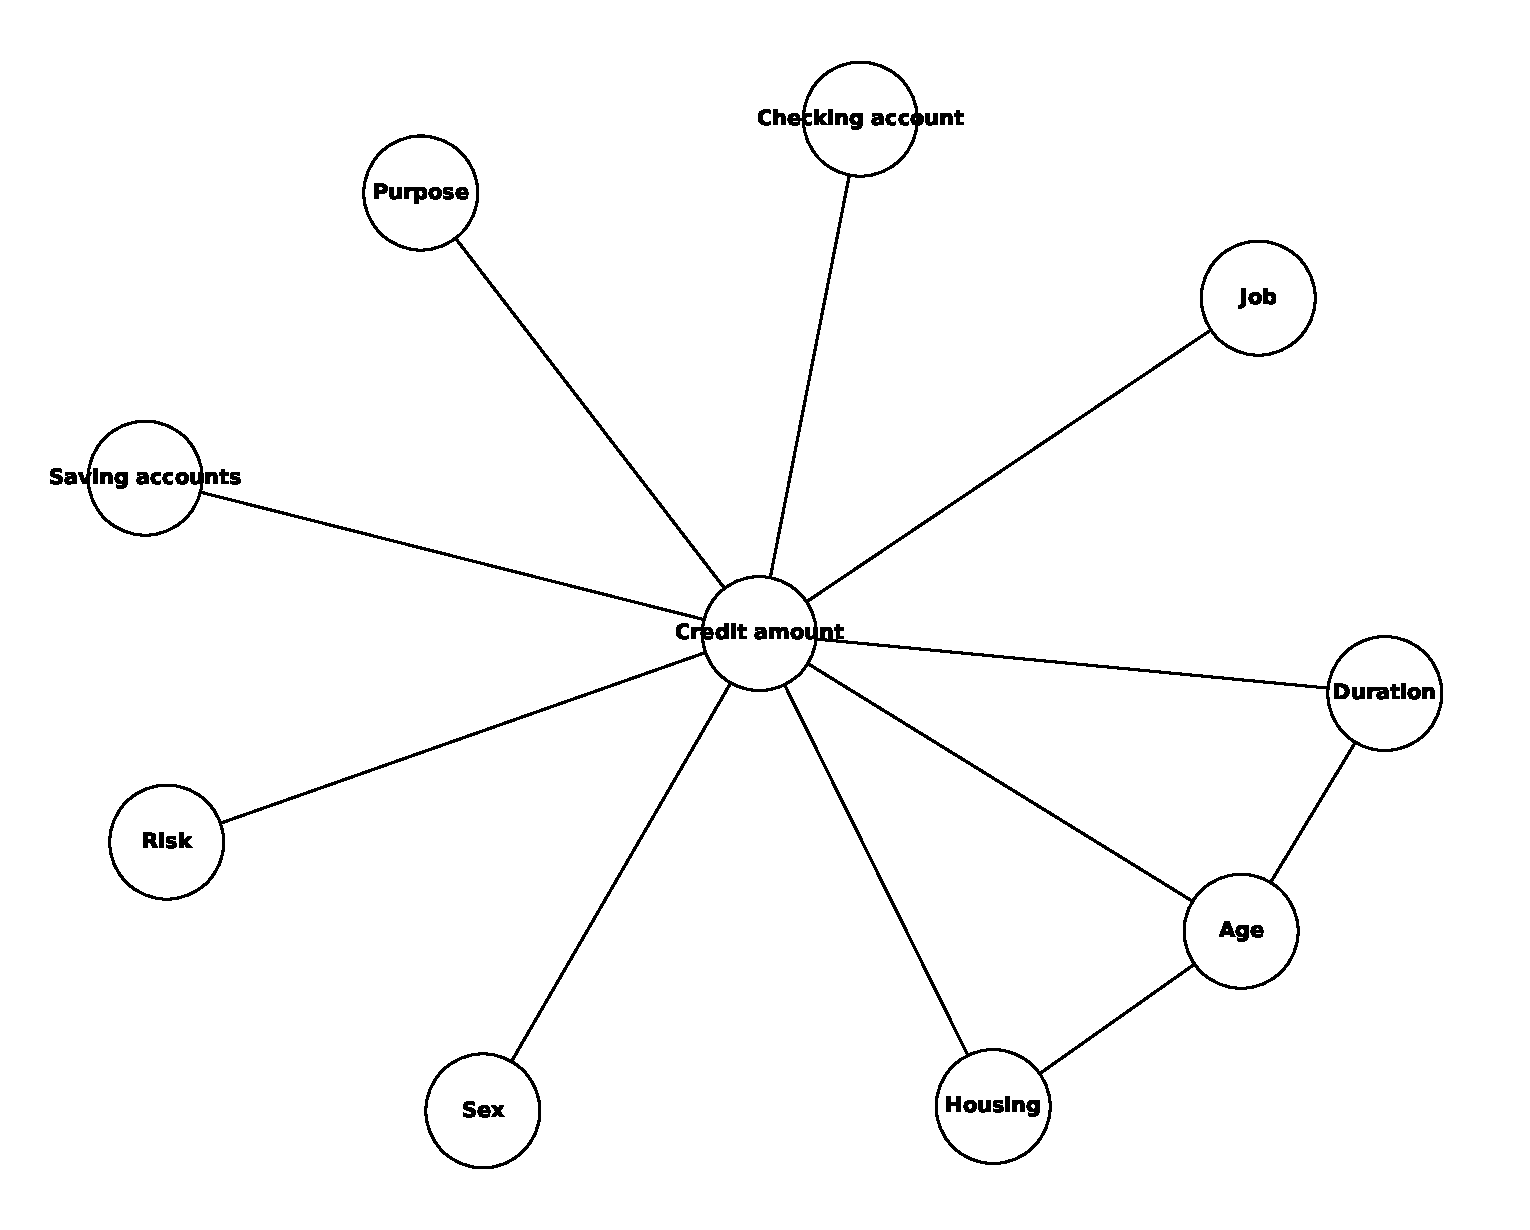
\includegraphics[width=\linewidth]{adult_mst}
%   \caption{Markov random field for marginals of the adult dataset.}
%   \label{fig:adult_mst}
%   \Description{Markov random field for marginals of the adult dataset.}
% \end{figure}

% \begin{figure}[h]
%   \centering
%   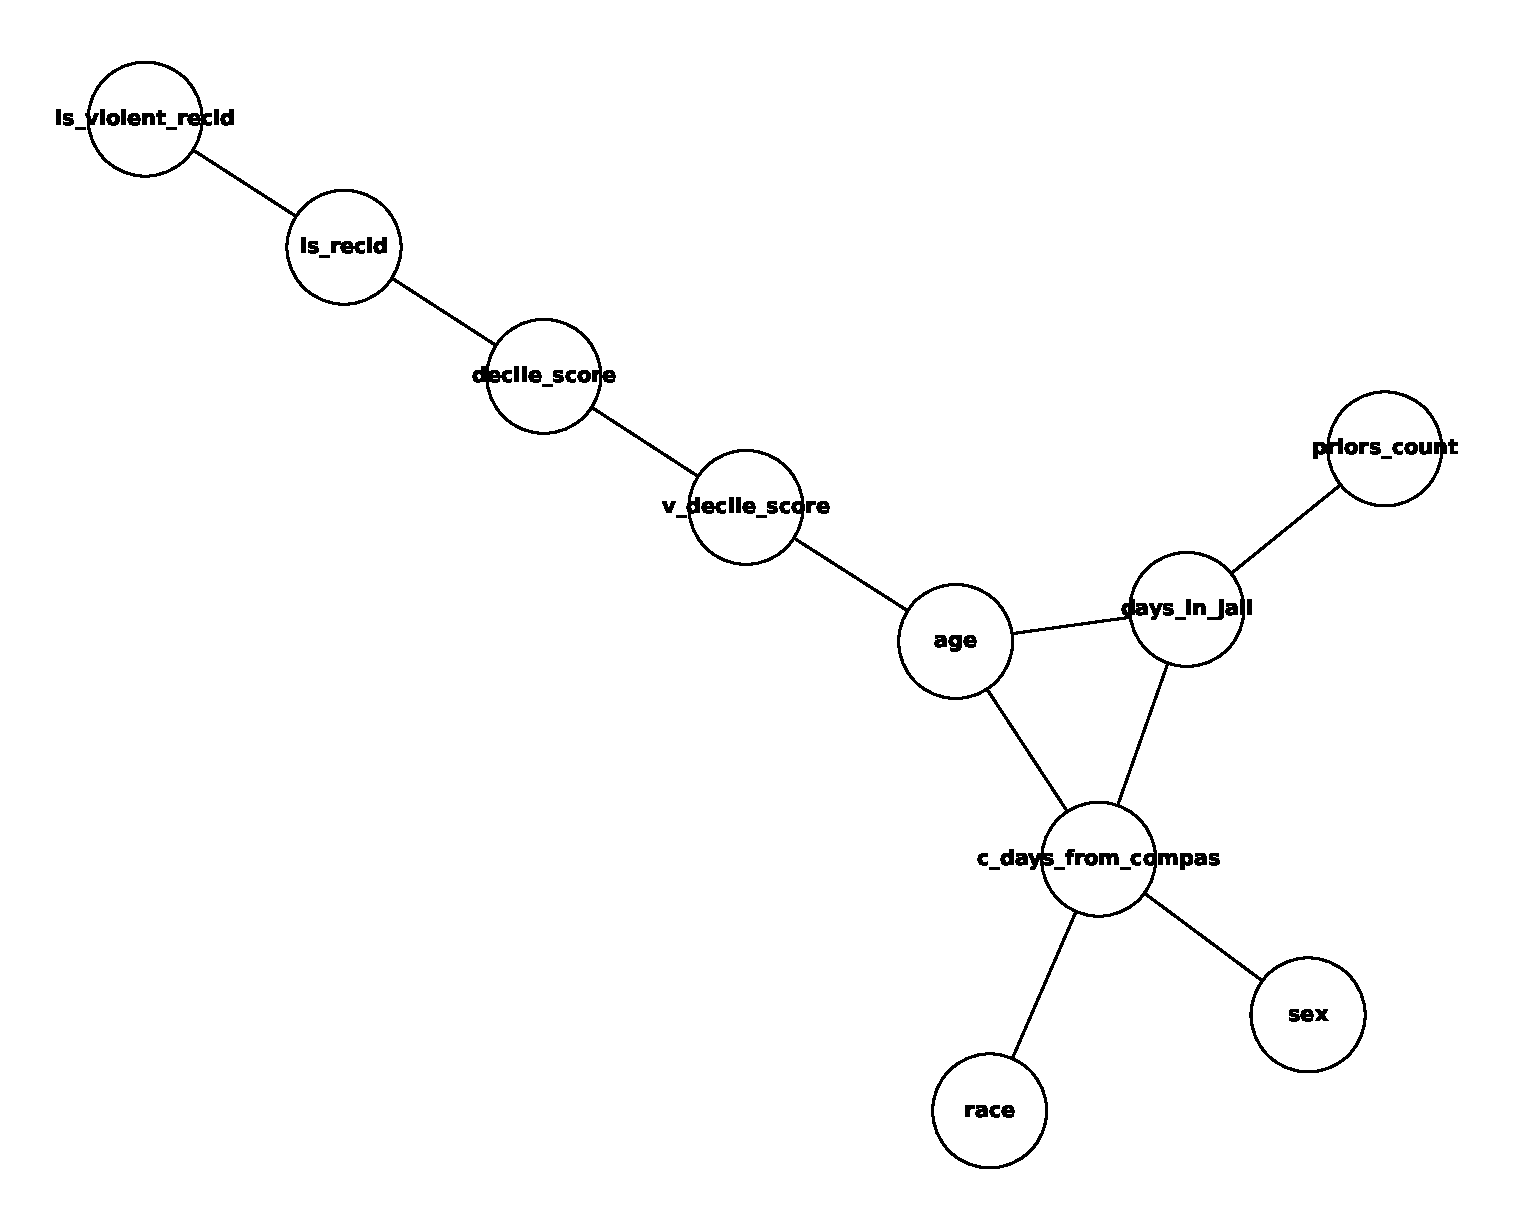
\includegraphics[width=\linewidth]{compas_mst}
%   \caption{Markov random field for marginals of the COMPAS dataset.}
%   \label{fig:compas_mst}
%   \Description{Markov random field for marginals of the COMPAS dataset.}
% \end{figure}

% \begin{figure}[h]
%   \centering
%   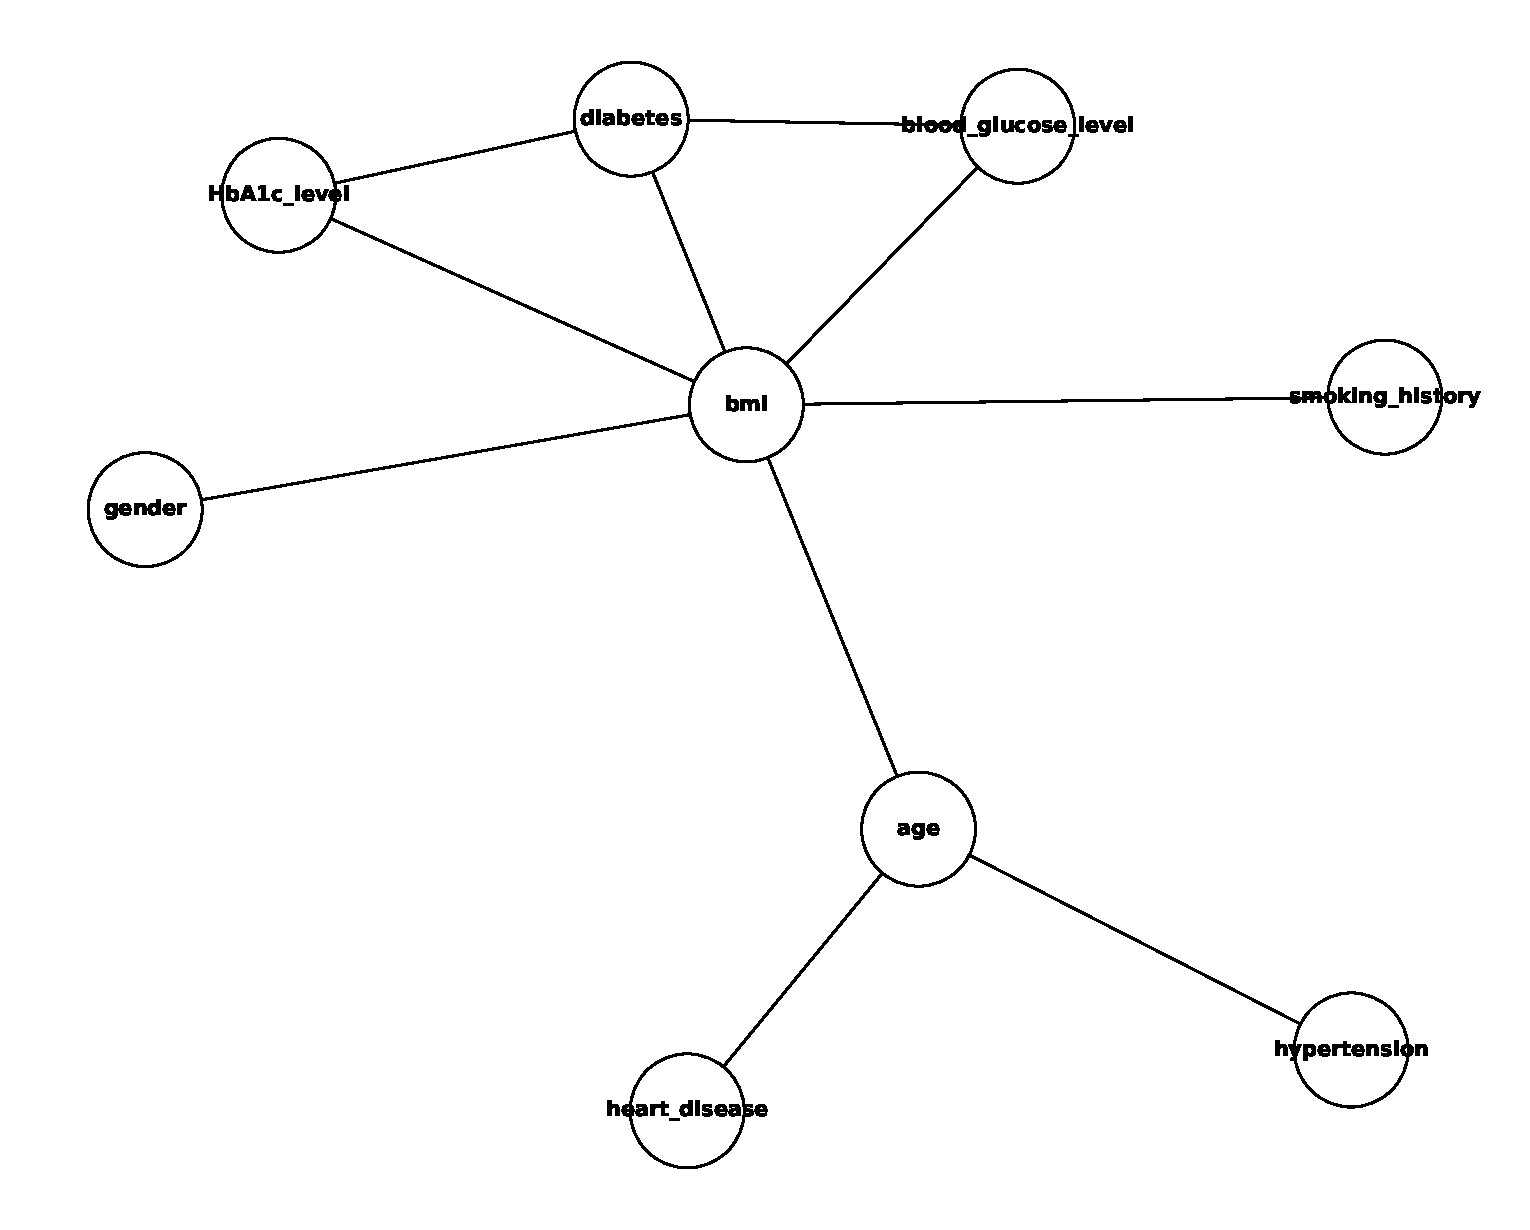
\includegraphics[width=\linewidth]{diabetes_mst}
%   \caption{Markov random field for marginals of the diabetes dataset.}
%   \label{fig:diabetes_mst}
%   \Description{Markov random field for marginals of the COMPAS dataset.}
% \end{figure}

\begin{figure}
  \centering
  \begin{subfigure}[b]{0.3\textwidth}
      \centering
      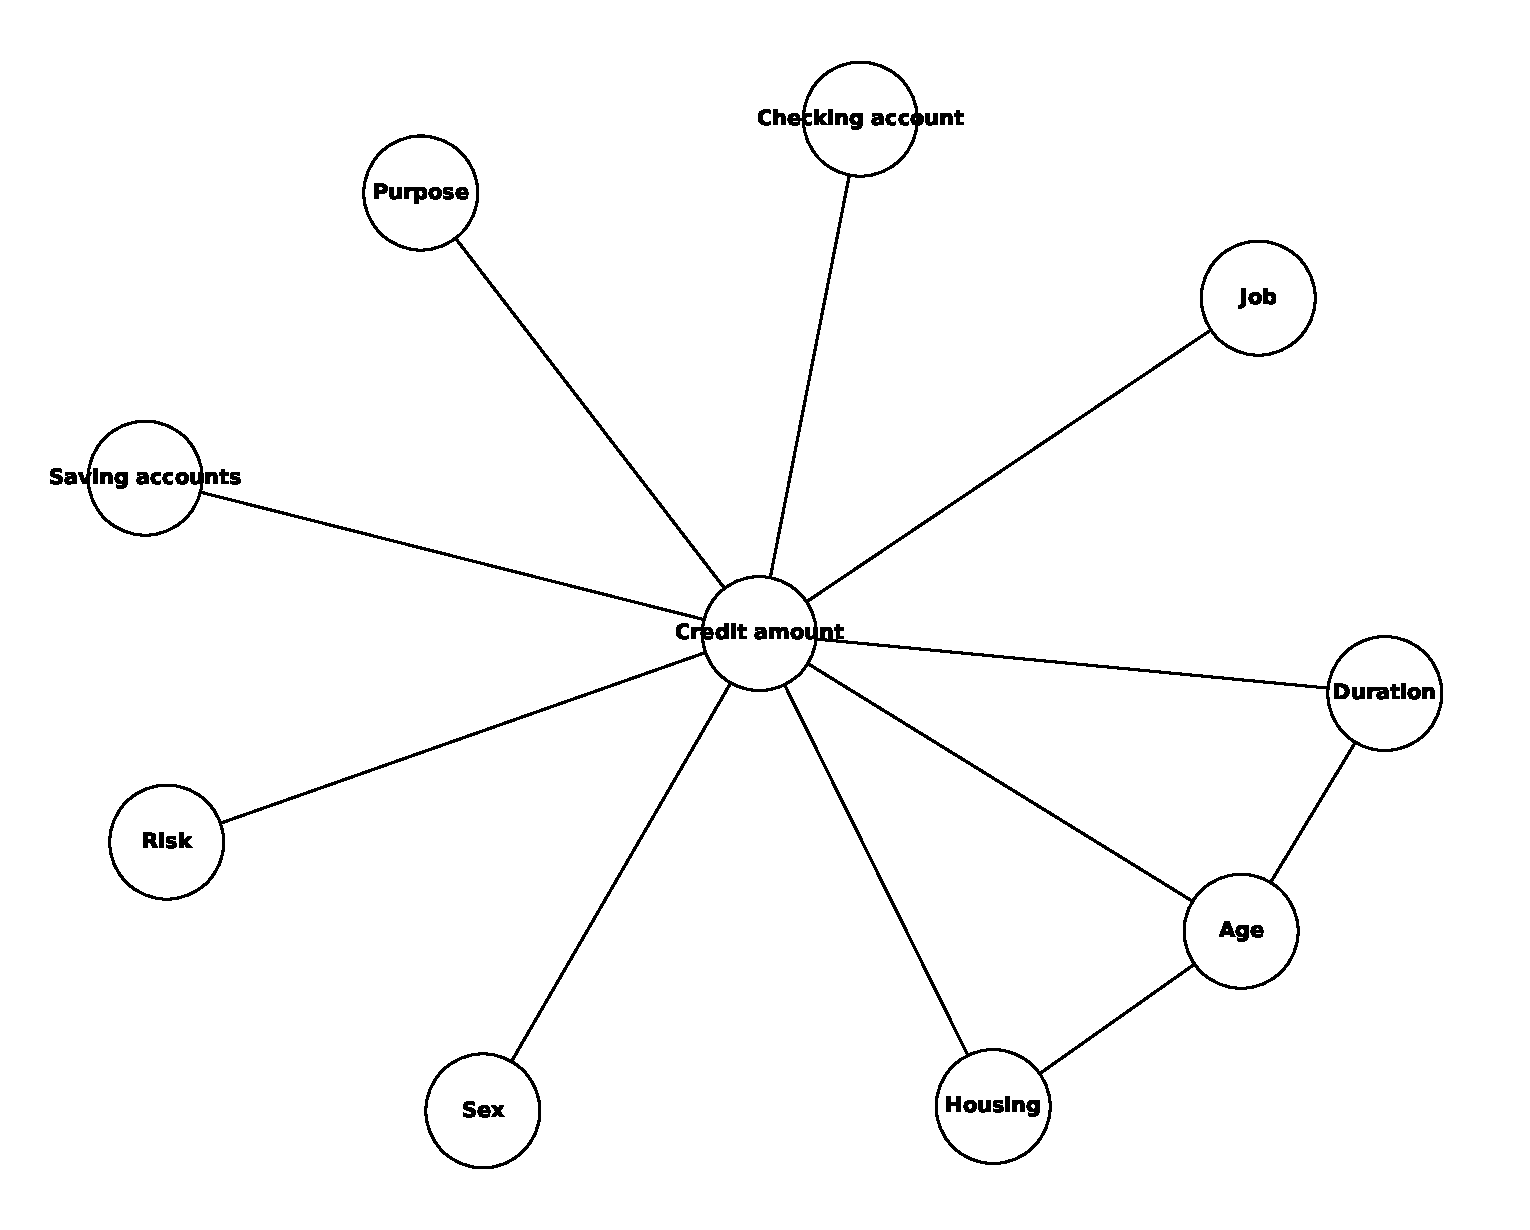
\includegraphics[width=\textwidth]{adult_mst}
      \caption{Markov random field for marginals of the adult dataset.}
      \label{fig:adult_mst}
      \Description{Markov random field for marginals of the adult dataset.}
  \end{subfigure}
  \hfill
  \begin{subfigure}[b]{0.3\textwidth}
      \centering
      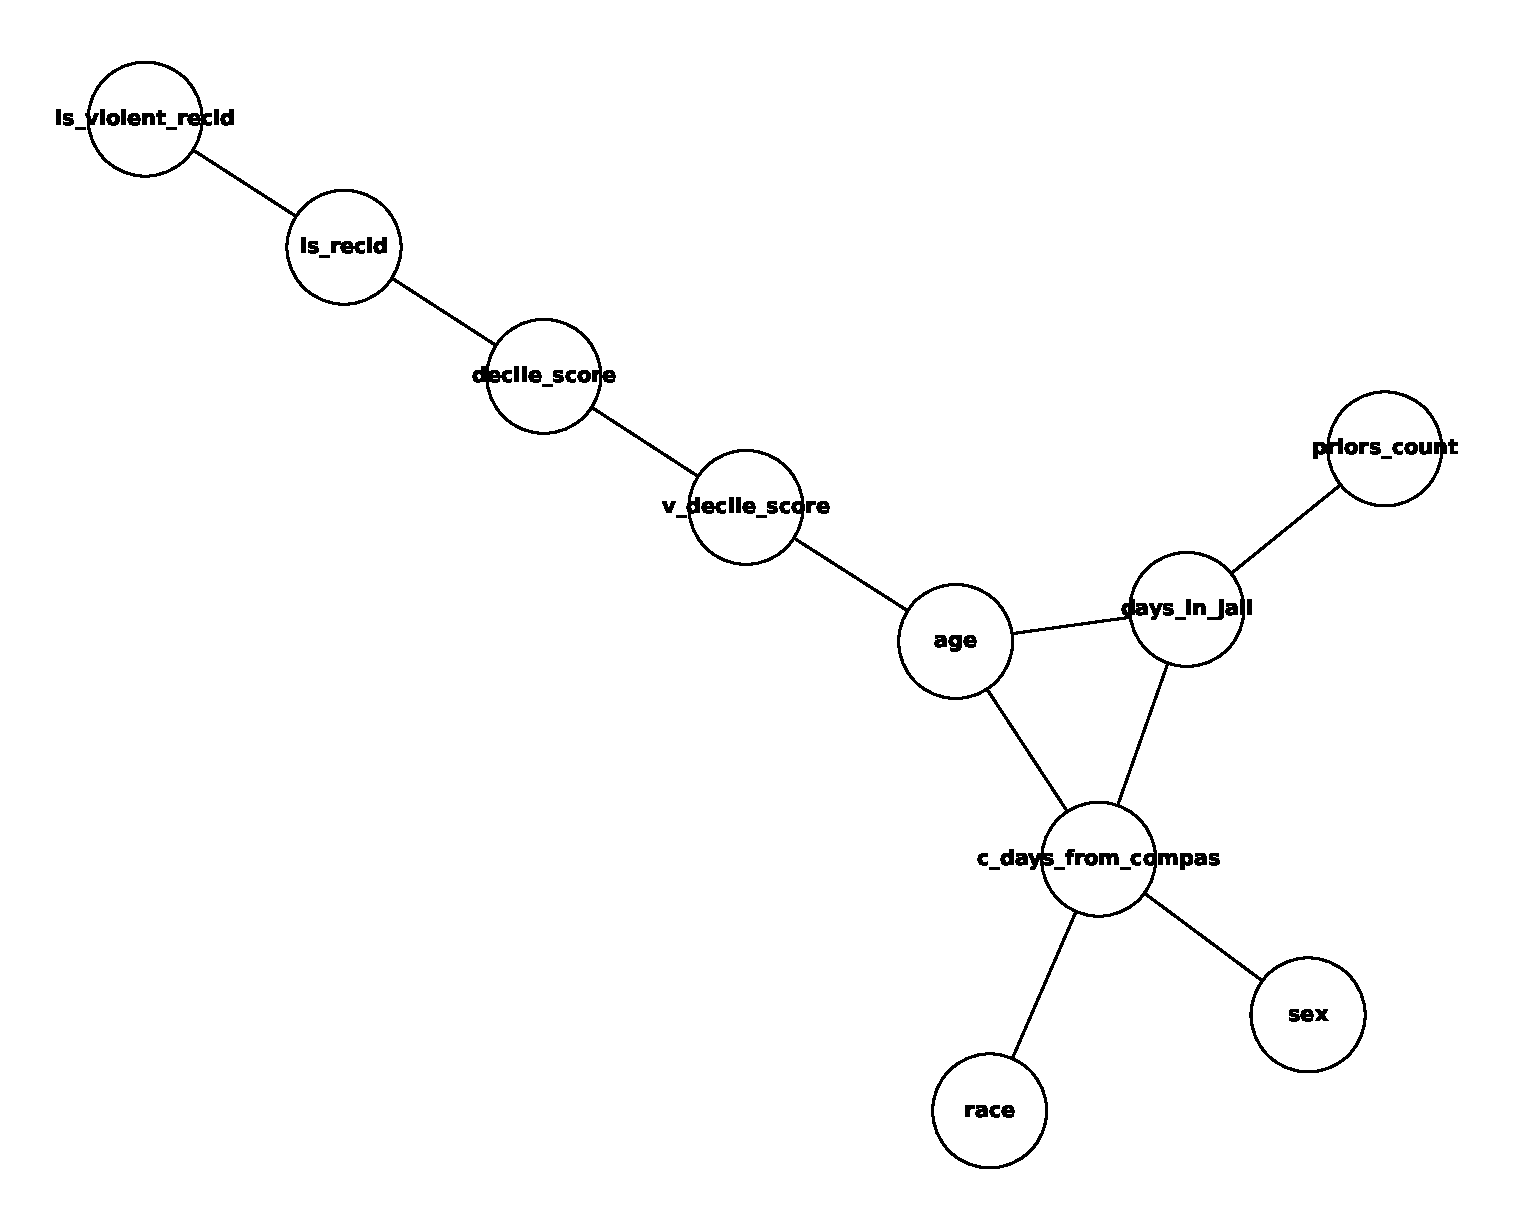
\includegraphics[width=\textwidth]{compas_mst}
      \caption{Markov random field for marginals of the COMPAS dataset.}
      \label{fig:compas_mst}
      \Description{Markov random field for marginals of the COMPAS dataset.}
  \end{subfigure}
  \hfill
  \begin{subfigure}[b]{0.3\textwidth}
      \centering
      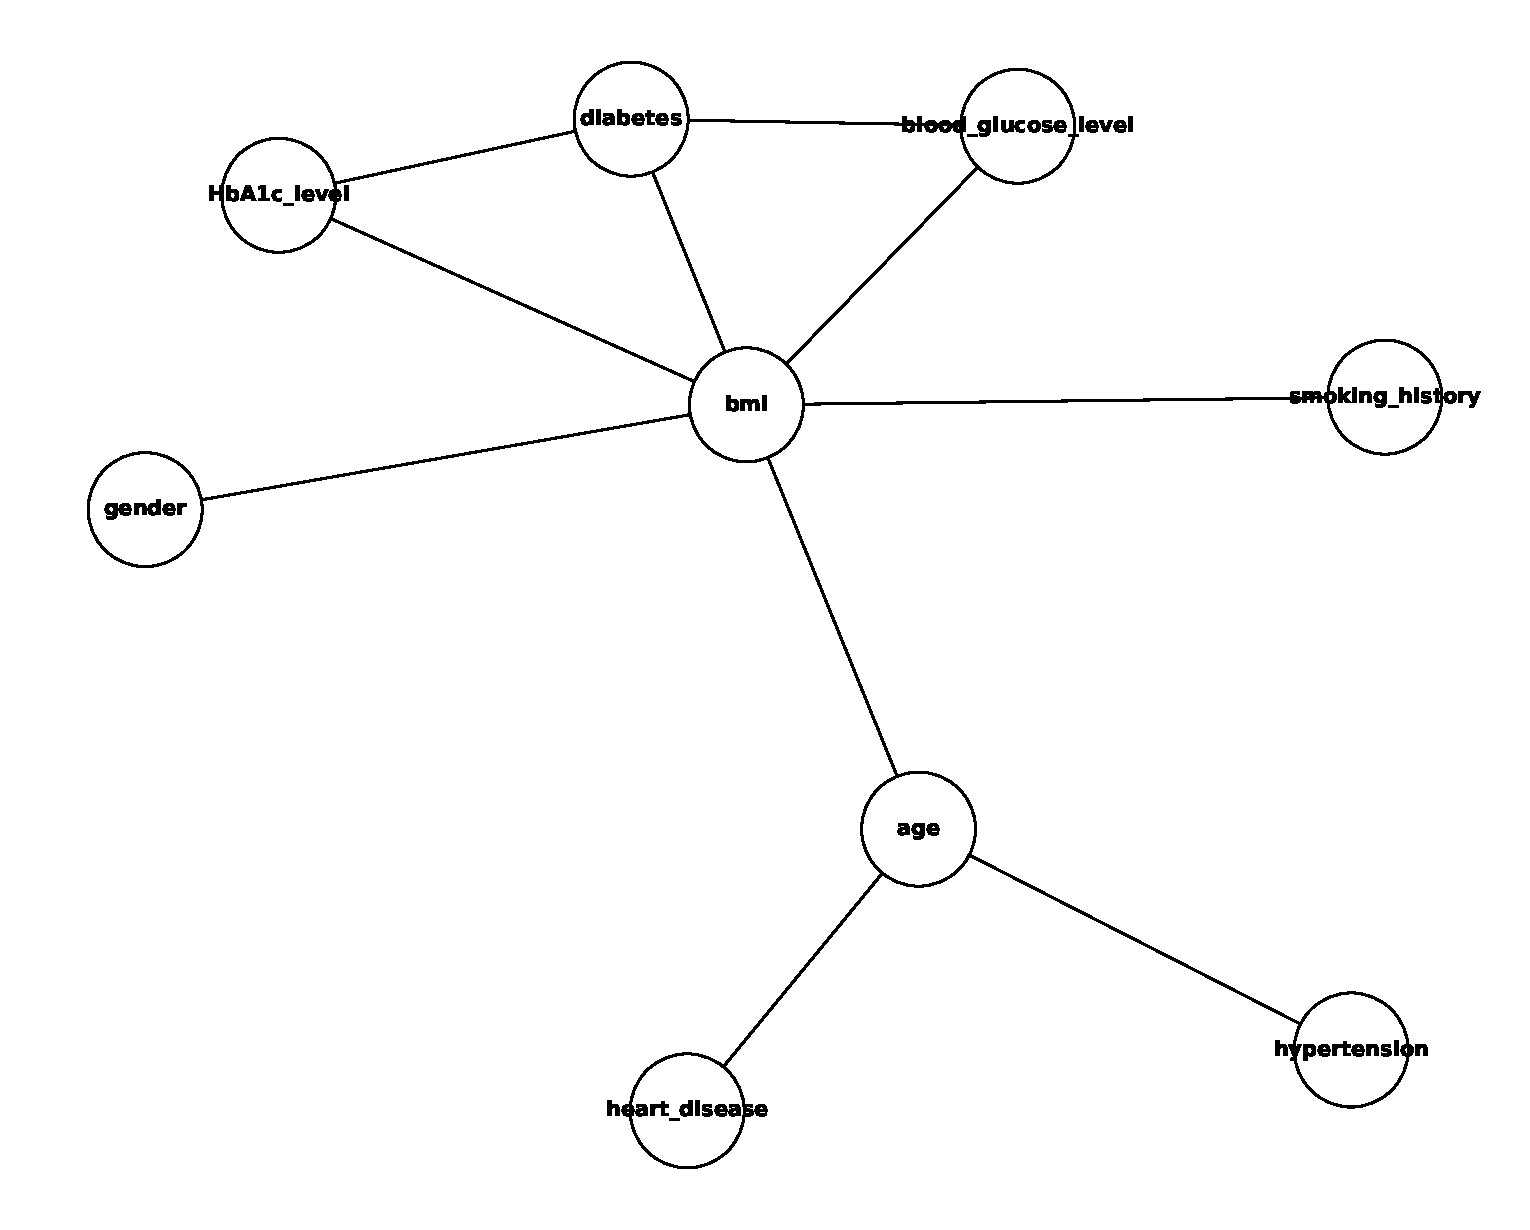
\includegraphics[width=\textwidth]{diabetes_mst}
      \caption{Markov random field for marginals of the diabetes dataset.}
      \label{fig:diabetes_mst}
      \Description{Markov random field for marginals of the COMPAS dataset.}
  \end{subfigure}
      \caption{Markov random field for marginals of the experimented datasets.}
      \label{fig:msts}
\end{figure}

% \begin{table}[h]
% \caption{Example marginals.}
% \label{tab:marginal-example}
% \centering
% \begin{subtable}[t]{0.3\linewidth}
%   \caption{Fairness measures experiment results of the adult dataset. Average of differences is 0.0431.}
%   \label{tab:adult_score}
%   \begin{tabular}{ccccc}
%   \toprule
%   \textbf{Measure} & \textbf{Original} & \textbf{Synthetic} & \textbf{Difference} \\
%   \midrule
%   Demographic Parity  & 0.172 & 0.104 & 0.067 \\
%   Accuracy Eqaulity   & 0.047 & 0.117 & 0.069 \\
%   Equalized Odds 1    & 0.057 & 0.079 & 0.021 \\
%   Equalized Odds 2    & 0.166 & 0.122 & 0.044 \\
%   Accuracy Equality 1 & 0.100 & 0.132 & 0.031 \\
%   Accuracy Equality 2 & 0.119 & 0.146 & 0.027 \\
%   \bottomrule
%   \end{tabular}
% \end{subtable}
% \begin{subtable}[t]{0.3\linewidth}
%   \centering
%   \caption{Fairness measures experiment results of the COMPAS dataset. Average of differences is 0.031.}
%   \label{tab:diabetes_score}
%   \begin{tabular}{cccc}
%   \toprule
%   \textbf{Measure} & \textbf{Original} & \textbf{Synthetic} & \textbf{Difference} \\
%   \midrule
%   Demographic Parity  & 0.013 & 0.015 & 0.002 \\
%   Accuracy Eqaulity   & 0.007 & 0.009 & 0.002 \\
%   Equalized Odds 1    & 0.000 & 0.003 & 0.003 \\
%   Equalized Odds 2    & 0.008 & 0.106 & 0.097 \\
%   Accuracy Equality 1 & 0.013 & 0.097 & 0.084 \\
%   Accuracy Equality 2 & 0.021 & 0.020 & 0.001 \\
%   \bottomrule
%   \end{tabular}
% \end{subtable}
% \end{table}

\subsection{Adult Income Dataset}

For the adult income dataset, the shape of the maximum spanning tree is very shallow, almost resembling a star; it has one internal node and all but one of the leaves have a depth of one. After introducing edges according to our heuristic, we observed an increase in the pairwise edges of the leaves, forming many 3-cliques and two 4-cliques. The resulting graph is shown in Figure~\ref{fig:adult_mst}.

Marginals based on this graph are then passed to the synthetic data generator for model fitting.

After generating ten rounds of synthetic data and passing them to the checker, their fairness measure values are averaged. Then, we compare them against the values of the original data. The results are shown in Table~\ref{tab:adult_score}.

% this 100 experiment is running

The fit time is 17m1s without heuristic. With heuristic it is 924m15s.

The average of their differences is $0.0787$. Without heuristic it is $0.0775$.

We observed that across all examined fairness measures, their difference all fall below 0.1. The average of their differences is 0.0431, which we consider quite satisfactory.

\begin{table}[h]
\caption{Fairness measures experiment results of the adult dataset. Average of differences is 0.0431.}
\label{tab:adult_score}
\begin{tabular}{ccccc}
\toprule
\textbf{Measure} & \textbf{Original} & \textbf{Synthetic} & \textbf{Difference} \\
\midrule
Demographic Parity  & 0.172 & 0.104 & 0.067 \\
Accuracy Eqaulity   & 0.047 & 0.117 & 0.069 \\
Equalized Odds 1    & 0.057 & 0.079 & 0.021 \\
Equalized Odds 2    & 0.166 & 0.122 & 0.044 \\
Accuracy Equality 1 & 0.100 & 0.132 & 0.031 \\
Accuracy Equality 2 & 0.119 & 0.146 & 0.027 \\
\bottomrule
\end{tabular}
\end{table}

\subsection{COMPAS Dataset}

For the COMPAS dataset, the initial spanning tree has a long tail, which is not surprising because, upon closer inspection, they all are related to the original COMPAS risk scores. The heuristic edge addition did not change the graph significantly. It only introduced one 3-clique triangle. The resulting graph is shown in Figure~\ref{fig:compas_mst}.

Marginals of this graph are then too passed to the synthetic data generator for fitting.

We ran the same workflow as adult dataset for the COMPAS dataset. The comparison results are shown in Table~\ref{tab:compas_score}.

% this experiment is complete

The fit time is 33s without heuristic. With heuristic it is 27m33s.

The average of their differences is $0.0750$. Without heuristic it is $0.0727$.

The results showed an increase in error on the sufficiency measure values. In particular, one of the measures has an error difference as high as 0.141. The average of their differences is 0.069, which is worse than the adult dataset.

\begin{table}[h]
\caption{Fairness measures experiment results of the COMPAS dataset. Average of differences is $0.0750$. Average of differences without heuristic is $0.0727$}
\label{tab:compas_score}
\begin{tabular}{cccccc}
\toprule
\textbf{Measure} & \textbf{Original} & \textbf{Synthetic} & \textbf{Difference} & \textbf{Synthetic(No Heuristic)} & \textbf{Difference(No Heuristic)} \\
\midrule
Demographic Parity  & 0.1310 & 0.0980 & 0.0330 & 0.0809 & 0.0501 \\
Accuracy Eqaulity   & 0.0079 & 0.0129 & 0.0050 & 0.0146 & 0.0067 \\
Equalized Odds 1    & 0.0249 & 0.0936 & 0.0687 & 0.0802 & 0.0553 \\
Equalized Odds 2    & 0.0177 & 0.1016 & 0.0838 & 0.0825 & 0.0648 \\
Accuracy Equality 1 & 0.1709 & 0.0505 & 0.1203 & 0.0551 & 0.1157 \\
Accuracy Equality 2 & 0.1695 & 0.0303 & 0.1392 & 0.0256 & 0.1439 \\
\bottomrule
\end{tabular}
\end{table}

\subsection{Diabetes Dataset}

The tree grown from the diabetes dataset did not appear to have any particular characteristics. The root of the tree is placed in the BMI value, which reasonably captures most information. The heuristic edge addition process introduced some 3-clique triangles. The resulting graph is shown in Figure~\ref{fig:diabetes_mst}.

The same process is conducted to fit the synthetic data generator model.

The same workflow was done as on previous datasets. The comparison results are shown in Table~\ref{tab:diabetes_score}.

% this experiment is complete

The fit time is 1m24s without heuristic. With heuristic it is 1m44s.

The average of their differences is $0.0067$. Without heuristic it is $0.0078$.

% The results showed that the synthetic data generally preserves the fairness properties of the original data.

% The average of the differences between the fairness measure values of the original and synthetic datasets is below 0.1 for all datasets. The average of the differences is 0.0431 for the adult dataset, 0.069 for the COMPAS dataset, and 0.031 for the diabetes dataset.

\begin{table}[h]
\caption{Fairness measures experiment results of the diabetes dataset. Average of differences is $0.0067$. Average of differences without heuristic is $0.0078$}
\label{tab:diabetes_score}
\begin{tabular}{cccccc}
\toprule
\textbf{Measure} & \textbf{Original} & \textbf{Synthetic} & \textbf{Difference} & \textbf{Synthetic(No Heuristic)} & \textbf{Difference(No Heuristic)} \\
\midrule
Demographic Parity  & 0.0135 & 0.0038 & 0.0096 & 0.0015 & 0.0119 \\
Accuracy Eqaulity   & 0.0077 & 0.0011 & 0.0065 & 0.0011 & 0.0065 \\
Equalized Odds 1    & 0.0000 & 0.0006 & 0.0006 & 0.0010 & 0.0010 \\
Equalized Odds 2    & 0.0086 & 0.0106 & 0.0020 & 0.0094 & 0.0008 \\
Accuracy Equality 1 & 0.0133 & 0.0090 & 0.0042 & 0.0059 & 0.0074 \\
Accuracy Equality 2 & 0.0216 & 0.0041 & 0.0175 & 0.0019 & 0.0197 \\
\bottomrule
\end{tabular}
\end{table}

\section{Evaluation}

% TODO: mention model fit time? yes. do experiments!

\subsection{Positive Results}

%  TODO: rewrite this

Our experiments showed that synthetic data generally preserves the fairness properties with a reasonable degree of accuracy. The average of the differences between the fairness measure values of the original and synthetic datasets is below 0.1 for all datasets. This indicates that synthetic data is a good approximation of the original data in terms of fairness.

For the adult dataset, the average difference was 0.0431, suggesting a close match between the synthetic and the original data in terms of fairness measures. For the diabetes dataset, the average difference was 0.031, which is even lower. Even in the case of the COMPAS dataset, which had a higher value, it was still within an acceptable range at 0.069.

In particular, both the independence and separation measures showed low errors across all datasets, with the differences of all of them below 0.1. On the other hand, results of accuracy equality also showed low errors, with the differences of one of them as low as 0.005.

This demonstrated that synthetic data can accurately reflect the fairness properties of the original data. Therefore, fairness analyses performed on synthetic data will yield results consistent with those on the original data.

\subsection{Negative Results}

%  TODO: rewrite this

The experiments also revealed some limitations of this approach. In particular, the sufficiency measure showed higher errors compared to other measures. For example, in the COMPAS dataset, the sufficiency measure had an error difference as high as 0.141, while other measures had errors below 0.1.

By close examination of our scenario, we can observe the following: of the three variables, $(\hat{Y},Y,S)$, two of them, namely $(Y,S)$, are both readily available in the original data. In contrast, $\hat{Y}$ is only available in the output of the given AI model, which cannot be captured by the synthetic data at the time of generation.

Referring back to the definition of the fairness measures, we can see the following: separation is concerned with the form $P[\hat{Y} | S, Y] = \frac{P[\hat{Y} \cap S \cap Y]}{P[{S} \cap Y]}$, and sufficiency is concerned with the form $P[Y | S, \hat{Y}] = \frac{P[Y \cap S \cap \hat{Y}]}{P[{S} \cap \hat{Y}]}$.

TODO: expand all defs and count the nums of avail vars

This explains why sufficiency measures could have higher errors compared to separation because synthetic data have less information about them. While only one variable is missing in the numerator for separation, one more variable is missing in the denominator for sufficiency.

Therefore, it is harder to approximate sufficiency measures on synthetic data. This is a fundamental limitation of this approach, and it is important to be aware of this when interpreting the results of fairness analyses.

% independence
% \[
% P[\hat{Y} | S] - P[\hat{Y} | \overline{S}]
% = \frac{P[\hat{Y} \cap S]}{P[{S}]} - \frac{P[\hat{Y} \cap \overline{S}]}{P[\overline{S}]}
% \]

% separation
% \[
% P[\hat{Y} | S, Y] - P[\hat{Y} | \overline{S}, Y]
% = \frac{P[\hat{Y} \cap S \cap Y]}{P[{S} \cap Y]} - \frac{P[\hat{Y} \cap \overline{S} \cap Y]}{P[\overline{S} \cap Y]}
% \]

% sufficiency
% \[
% P[Y | S, \hat{Y}] - P[Y | \overline{S}, \hat{Y}]
% = \frac{P[Y \cap S \cap \hat{Y}]}{P[{S} \cap \hat{Y}]} - \frac{P[Y \cap \overline{S} \cap \hat{Y}]}{P[\overline{S} \cap \hat{Y}]}
% \]

\section{Conclusion}


%%
%% The acknowledgments section is defined using the "acks" environment
%% (and NOT an unnumbered section). This ensures the proper
%% identification of the section in the article metadata, and the
%% consistent spelling of the heading.
% \begin{acks}
% To Robert, for the bagels and explaining CMYK and color spaces.
% \end{acks}

%%
%% The next two lines define the bibliography style to be used, and
%% the bibliography file.
\bibliographystyle{ACM-Reference-Format}
\bibliography{references}


%%
%% If your work has an appendix, this is the place to put it.
% \appendix

\end{document}
\endinput
%%
%% End of file `sample-manuscript.tex'.
